欢迎大家。

今天我将讲解线程束分化（Warp Divergence），因为如果您想优化 CUDA 应用程序，这是一个非常重要的主题。按照惯例，我将首先回顾之前关于线程束（Warp）、线程（Thread）和线程块（Block）的讨论内容。

我们知道，线程被组织在线程块中，而线程块又进一步划分为线程束。我们还知道，一个线程束由 32 个线程组成，这些线程可以在单条指令下同时执行。这被称为 SIMT（单指令多线程）模型，意味着我们可以使用多个线程（此处为 32 个线程）对不同的数据元素执行同一条指令。

大家是否还记得向量加法示例？如图所示，我们只有一条指令，即加法运算。但我们正在使用多个线程执行这条单一指令，正如公式所示，这里利用了与线程 ID 相关的索引值。也就是说，我们使用多个线程对数组 A 和 B 中的不同元素执行同一条加法指令。这很简单，这就是所谓的 SIMD（单指令多数据）模型。

但我们也知道，每个线程束都由一个指令调度器控制。大家是否还记得流多处理器（SM）内部的组件？复习这些内容非常重要。

这张图展示了流多处理器（SM）内部的所有组件。如图所示，SM 包含多个分区，每个分区可以同时执行一个线程束。此外还有 L1 数据缓存、共享内存、纹理内存等其他组件。但我在此重点关注的是线程束调度器，即线程束的管理器。因为在大多数应用中，流多处理器中可能需要执行大量线程束，因此需要一个管理器将这些线程束调度到可用的硬件资源（即硬件核心）上。

这里需要重点关注的核心概念是：理想情况下，每个时钟周期可以发射 32 个线程。请注意，这 32 个线程执行的是同一条指令（例如加法运算），而不是 32 条不同的指令。它们利用不同的计算单元同时执行。这就是理想场景：线程束中的所有 32 个线程同时执行相同的指令，正如前面的示例所示。

然而，如果存在 if-else 语句，不同的线程可能会走不同的执行路径，这就导致了线程束分化。

请看这个例子。这里有一个边界检查语句，另一个是条件判断语句。前者不会导致线程束分化，因为其条件仅涉及向量的边界检查。例如，若向量大小为 1024 个元素，该条件仅在最后一个线程中触发，而不会在线程束内的多个线程中同时触发。该检查旨在确保我们不处理超出向量范围的元素。当向量大小不是 32 的倍数时（例如大小为 1000），这种检查是必需的。由于线程数量必须是 32 的倍数，我们需要启动 1024 个线程，但实际只需处理 1000 个元素，因此必须通过条件判断禁止 ID 大于等于 1000 的线程执行计算。

相比之下，第二个 if-else 语句则会导致分化。该语句判断索引值是否小于 16，这一条件可能在一个或多个线程束内的多个线程中同时成立或失败。因此，这被称为线程束分化（而非线程块分化或线程分化）。在这种情况下，同一个线程束中的部分线程将执行 if 分支，而其他线程将执行 else 分支。只有当所有线程都完成各自的分支执行后，才会汇合执行后续的加法操作。

简而言之，当应用程序中存在 if-else 语句且导致同一线程束内的线程走向不同路径时，就会发生线程束分化。最关键的一点是：当发生线程束分化时，GPU 会串行化执行不同的分支。这意味着执行不同分支的线程无法同时运行，而是必须分步执行：先执行第一个分支，再执行第二个分支，最后才执行汇合后的加法操作。这与无分化的理想场景截然不同，在理想场景中所有线程同时执行加法操作。因此，如果应用程序中存在严重的线程束分化，将会导致性能下降。

\begin{figure}
    \centering
    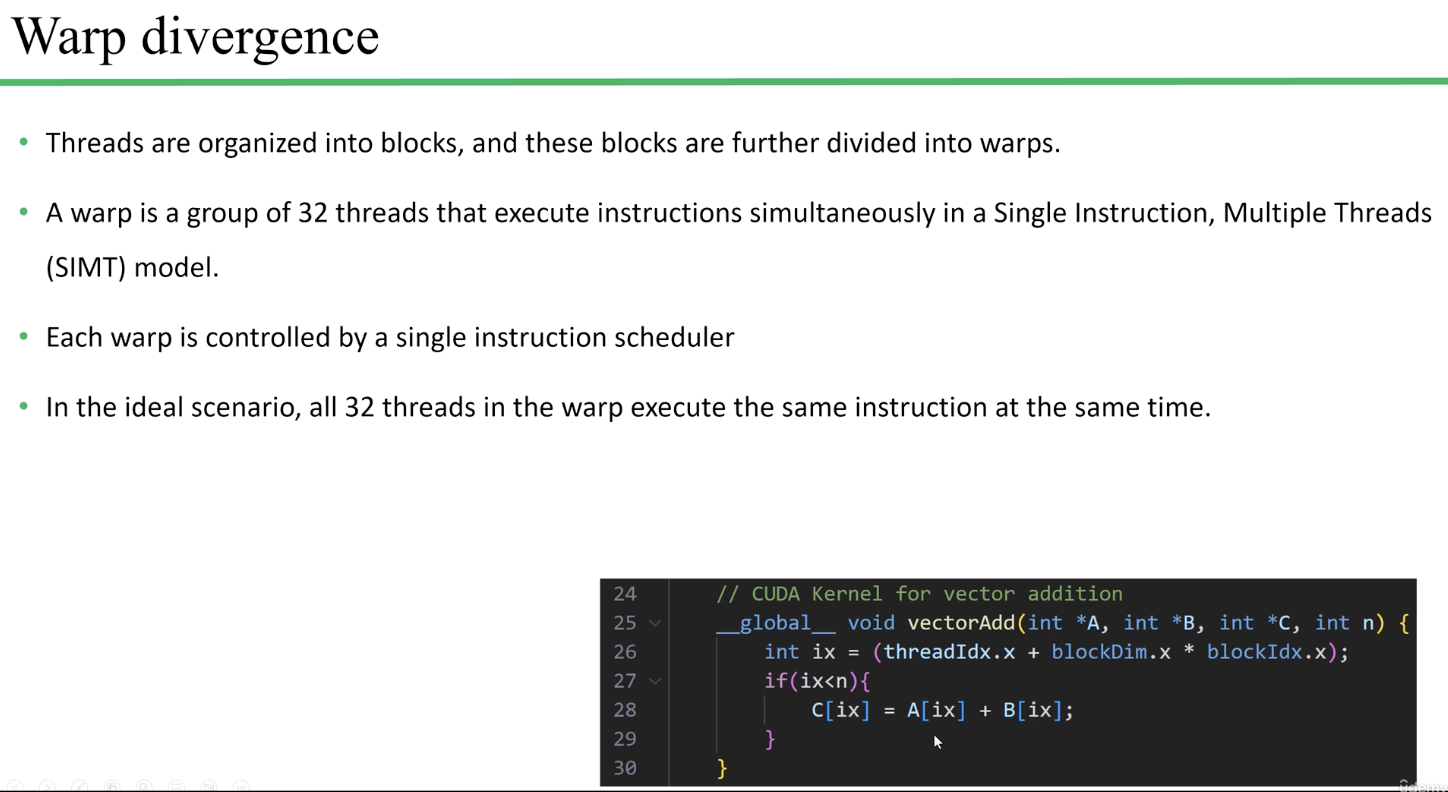
\includegraphics[width=0.75\linewidth]{resources/cuda-128.png}
    \caption{}
    \label{fig:placeholder}
\end{figure}

下面通过几个示例进一步说明：

无线程束分化：线程束中的所有 32 个线程执行相同的路径，没有任何分支。这是 SIMT 的理想场景，性能最优，因为所有线程同时执行，通常在 1 到 2 个时钟周期内完成，且所有线程均处于活跃状态。
中度线程束分化：半数线程走一个分支，另一半线程等待。例如，前 16 个线程执行路径 A，此时后 16 个线程处于停滞（Idle）状态；待路径 A 执行完毕后，后 16 个线程再执行路径 B。由于只有一个层级的分化，故称为“中度”。在此过程中，部分线程处于空闲状态，降低了整体效率和线程束利用率。
严重线程束分化：当存在多个 if 语句，且每个语句都影响线程束内的部分线程时，就会发生这种情况。例如，根据线程索引的奇偶性或其他规则，将线程分为多组，每组执行不同的路径。这导致线程在不同分支间频繁切换，活跃与空闲状态交替出现。这是最糟糕的情况，因为在每个时钟周期内大多数线程都处于空闲状态，从而导致显著的性能损失。

接下来讨论线程束分化对性能的具体影响：

性能影响：如果线程发生分化，同一时刻只能执行一条路径，而线程束中的其他线程处于空闲状态，等待同步点。
串行化：分化的线程束导致多条路径被串行执行，降低了吞吐量，因为在任意给定时刻，只有部分线程束在执行有效工作。
资源利用低效：任意时刻只有部分线程在执行，非活跃线程实际上浪费了硬件资源。
执行时间增加：由于不同路径导致线程束执行被拆分为多个步骤，控制流的串行化迫使 GPU 在不同执行路径间切换，增加了内核的整体完成时间。
吞吐量降低：线程束分化导致每个时钟周期的活跃线程数减少，从而降低了指令吞吐量。

以上就是关于线程束分化的全部核心知识。我不打算在此处演示简单的向量加法优化示例，因为对于如此简单的应用，优化带来的性能提升并不显著。但在后续的“向量归约”章节中，您将看到优化线程束分化能带来显著的性能提升。

最后展示一个辅助理解的图示案例。假设有一个 if-else 语句，偶数线程执行一部分，奇数线程执行另一部分，最后统一执行乘法操作。32 个线程作为一个整体同时到达 if 语句并进行条件测试，但由于路径不同，它们将被串行执行。首先，部分线程进入第一条路径，其余线程通过掩码机制（Masking）被屏蔽并处于空闲状态；随后，剩余线程进入第二条路径执行，同样伴随掩码操作；最终，所有线程在 if 语句结束处汇合，共同执行最后一条指令。

这就是线程束分化的全部内容，这是一个非常重要的主题。今天的课程到此结束，下节课再见。
